\documentclass[11pt]{article}
\usepackage{amsmath}
%\usepackage{extsizes}
\usepackage{amsmath,amssymb}
%\usepackage{omegavn,ocmrvn}
%\usepackage[utf8x]{inputenc}
\usepackage[utf8]{vietnam}

\usepackage{longtable}
\usepackage{answers}
\usepackage{graphicx}
\usepackage{array}
\usepackage{pifont}
\usepackage{picinpar}
\usepackage{enumerate}
\usepackage[top=3.0cm, bottom=3.5cm, left=3.5cm, right=2.5cm] {geometry}
\usepackage{hyperref}


\usepackage{listings}
\lstset{language=Python}          % Set your language (you can change the language for each code-block optionally)


\newtheorem{bt}{Câu}
\newcommand{\RR}{\mathbb R}
\Newassociation{sol}{Solution}{ans}
\newtheorem{ex}{Câu}
\renewcommand{\solutionstyle}[1]{\textbf{ #1}.}
\newcommand{\m}[1]{
	\begin{bmatrix}
		#1
	\end{bmatrix}
}

\begin{document}
% \noindent
\begin{tabular*}
{\linewidth}{c>{\centering\hspace{0pt}} p{.7\textwidth}}
Trường ĐHKHTN, ĐHQGHN & {\bf Học Kỳ 1 (2020-2021)}
\tabularnewline
K63 TTƯD - MT\&KHTT \\ Lớp thầy Hà Phi & {\bf Bài kiểm tra giữa kỳ}
\tabularnewline
\rule{1in}{1pt}  \small  & \rule{2in}{1pt} %(Due date:)
\tabularnewline

%  \tabularnewline
%  &(Đề thi có 1 trang)
\end{tabular*}
%
% \Opensolutionfile{ans}[ans1]

\begin{center}	
\textbf{Các em có thể lựa chọn 1 trong các tổ hợp 123, 134, 234, 135, 235}
\end{center}

\begin{bt}(4 $\times$ 1 = 4 điểm) \\
a)	Chứng minh rằng phương trình $1+4x-10x^3=0$ có nghiệm duy nhất trong đoạn $[0.5, 1]$. \\
b)	Có rất nhiều các khác nhau để chuyển về bài toán tìm điểm bất động ($x=\varphi(x)$) để giải bằng phương pháp lặp đơn. Ta lấy ví dụ 2 phương pháp sau.
%
\[
i) \ \varphi(x) = 1+5x-10x^3 \ , \hskip 4cm \qquad ii) \ \varphi(x) = \sqrt{\dfrac{1+4x}{10x}} \ .
\]
%
Hãy biện luận về tính hội tụ của các phương pháp trên. \\
Hai câu sau chỉ thực hiện cho phương pháp ii) . \\
c) Tìm số bước lặp cần thiết sao cho sai số tuyệt đối của nghiệm bé hơn $1e-9$ với $x_0$ tùy chọn. \\
d) Tính $x_3$ chính xác đến 4 chữ số thập phân và đánh giá sai số hậu nghiệm cho $x_3$, với $x_0 = 0.8$. 
\end{bt}


\begin{bt}(4 $\times$ 1 = 4 điểm) \\
	a) Viết công thức lặp để giải hệ phương trình sau bằng phương pháp Jacobi. Phương pháp lặp này có hội tụ không? Vì sao?
	%
	\begin{align*}
	4 x_1 + 0.4 x_2 - 0.4 x_3 &= 8 \\
	0.3 x_1 - 3 x_2 - 0.6 x_3 &= -9 \\
	0.5 x_1 + 0.5 x_2 - 5 x_3 &= 5 
	\end{align*}
	%
	b) Đối với hệ $x^{i+1} = M x^{i} + n$ mà các em vừa thu được bằng phương pháp Jacobi, hãy tìm $\|\cdot\|_1$ và $\|\cdot\|_{\infty}$ của ma trận hệ số $M$. \\
	c) Tính số bước lặp cần thiết bằng ước lượng tiên nghiệm sao cho ta có ước lượng sai số nghiệm $\|x^*-x^n\| \leq 1e-6$, với chuẩn $\|\cdot\|$ phù hợp và với $x^0$ tùy chọn. \\
	d) Cho $x^0 = \m{0 & 0 & 0}^T$. Hãy tìm $x^i$, $i=1,2,3$. Hãy sử dụng ước lượng hậu nghiệm để đánh giá sai số của $x_3$.
\end{bt}

\begin{bt}(2 điểm PLU + 2 điểm giải hệ) \\
Tìm phân tích PLU của ma trận 
\[
A = \m{2.34 & -4.10 &  1.78 \\
	1.98  & 3.47 &  -2.22 \\
	2.36  & -15.17 &  6.81}
\]
và hãy áp dụng để giải hệ sau
%
\[
\m{2.34 & -4.10 &  1.78 \\
	1.98  & 3.47 &  -2.22 \\
	2.36  & -15.17 &  6.81} 
\m{x_1 \\ x_2 \\ x_3} = \m{0.02 \\ 	-0.73 \\ -6.63}
\]
%
\end{bt}
\cleardoublepage

\begin{center}	
	\textbf{ Đề II - Thi trên máy 60 phút}
\end{center}

\begin{bt}(3 điểm) \\ % Exercise 22, Kiusalass p.170 
	Thùng dầu hình trụ có bán kính r và chiều dài L được đổ đầy đến độ sâu h. Kết quả
	khối lượng dầu trong thùng là
	\[
	V = r^2L \Big( \phi - \left(1 - \dfrac{h}{r}\right) sin \phi \Big)
	\]
	trong đó $\phi = arcos\left(1 - \dfrac{h}{r}\right)$. Nếu bể đầy 3/4, hãy xác định tỉ số $h/r$.
	
	\begin{figure}[h!]
		\centering
		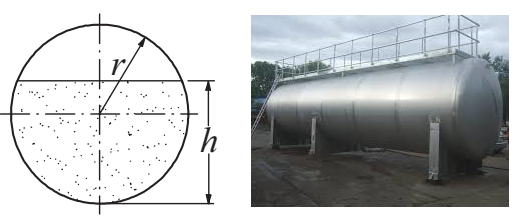
\includegraphics[width=0.7\linewidth]{oil_tank}
		\caption{}
		\label{fig:oiltank}
	\end{figure}
\end{bt}

\begin{bt}(3 điểm) \\
Hãy vẽ đồ thị hàm số và lập trình phương pháp Newton để tính toán tất cả các nghiệm thực dương của phương trình
\[ 
f(x) = x^4 + 2x^3 - 7x^2 + 3 = 0,
\]
với sai số $1e-9$. So sánh với nghiệm (giả sử chính xác) có được bằng cách sử dụng hàm fsolve \verb|from scipy.optimize import fsolve| và tính sai số tương đối.
\end{bt}

\centerline{———————————Hết——————————-}

\vspace{1cm}
\noindent{\bf Chú ý:} {\it Cán bộ coi thi không giải thích gì thêm}\\

  
\end{document}



